\chapter{Graphical user interface}\label{chapGUI}

This chapter presents our graphical user interface (GUI) to carry out Bayesian regression analysis in a very friendly environment without any programming skills (drag and drop). Our GUI is based on an interactive web application using \textit{shiny} \cite{Chang2018}, and packages like \textit{MCMCpack} \cite{Martin2018} and \textit{bayesm} \cite{Rossi2017} from \textbf{R} software \cite{R2023}, and is designed for teaching and applied purposes at an introductory level. In the next chapters of the second part of this book we carry out some applications to highlight the potential of our GUI for applied researchers and practitioners.

\section{Introduction}\label{secGUI1}

Our GUI allows performing inference using Bayesian regression analysis without requiring programming skills. The latter seems to be a significant impediment to increasing the use of the Bayesian framework \cite{Woodward2005,Karabatsos2016}.

There are other available graphical user interfaces for carrying out Bayesian regression analysis. \textit{ShinyStan} \cite{shinystan2017} is a very flexible open source program, but users are required to have some programming skills. \textit{BugsXLA} \cite{Woodward2005} is open source, but less flexible. However, users do not need to have programming skills. \textit{Bayesian regression: Nonparametric and parametric models} \cite{Karabatsos2016} is a very flexible and friendly GUI that is based on \textit{MATLAB Compiler} for a 64-bit Windows computer. Its focus is on Bayesian nonparametric regressions, and it can be thought of for users who have mastered basic parametric models, such as the ones that we show in our GUI. There are also \textit{MATLAB toolkit}, \textit{Stata} and \textit{BayES}, but these are not open sources.

We developed our GUI based on an interactive web application using shiny \cite{Chang2018}, and some libraries in \textbf{R} \cite{R2021}. The specific libraries and commands that are used in our GUI can be seen in Table \ref{tab:libraries}. It has ten univariate models, four multivariate, {\color{red}time series models}, three hierarchical longitudinal, and seven Bayesian model averaging frameworks. In addition, it gives basic summaries and diagnostics of the posterior chains, as well as the posterior chains themselves, and different plots, such as trace, autocorrelation and densities. 

In terms of its flexibility and possibilities, our GUI lies between \textit{ShinyStan} and \textit{BugsXLA}: users are not required to have any programming skills, but it is not as advanced as \cite{Karabatsos2016}'s software. However, our GUI can be run in any operating system. Our GUI, which we call BEsmarter,\footnote{Bayesian econometrics: Simulations, models and applications to research, teaching and encoding with responsibility.} is freely available at \textbf{https://github.com/besmarter/BSTApp}; so users have access to all our code and datasets. 

Simulated and applied datasets are in the folders \textbf{DataSim} (see Table \ref{tab:simdata} for details), and \textbf{DataApp} (see Table \ref{tab:appdata} for details) of our \textbf{GitHub} repository. The former folder also includes the files that were used to simulate different processes, so, the population parameters are available, and as a consequence these files can be used as a pedagogical tool to show some statistical properties of the inferential frameworks available in our GUI. The latter folder contains the datasets used in the applications of this second part of the book. Users should use these datasets as templates to structure their own datasets. 

There are three ways to install our GUI. The easiest way, but that requires installation of \textbf{R}, and potentially a \textbf{R} code editor, is to type

\begin{tcolorbox}[enhanced,width=4.67in,center upper,
	fontupper=\large\bfseries,drop shadow southwest,sharp corners]
	\textit{R code. How to display our graphical user interface}
	\begin{VF}
		\begin{lstlisting}[language=R]
		shiny::runGitHub("besmarter/BSTApp", launch.browser = T)\end{lstlisting}
	\end{VF}
\end{tcolorbox} 

in the \textbf{R} package console or any \textbf{R} code editor. We strongly recommend to type this directly, rather than copy and paste. This is due to a potential issue with the quotation mark. 

The second option is to visit \textbf{https://posit.cloud/content/4328505}, log in or sign up for \textbf{Posit Cloud}, and access the project titled \textbf{GUIded Bayesian regression app BSTApp}. In the right-bottom window, click on the \textbf{BSTApp-master} folder under \textbf{Files}, open the \textbf{app.R} file, and finally, click the \textbf{Run App} button. However, inactivity will cause the window to close.

The third approach, and our recommendation, is using a \textbf{Docker} image by running:
\begin{enumerate}
	\item docker pull magralo95/besmartergui:latest
	\item docker run --rm -p 3838:3838 magralo95/besmartergui  
\end{enumerate}
in your \textbf{Command Prompt}. This creates an isolated environment for our GUI, ensuring consistent performance across systems. Note that \textbf{Docker} must be installed to deploy our GUI this way.

After implementing any of the three ways to run our GUI, users can see a new window where a presentation of our research team is displayed (see Figure \ref{fig61}). In addition, the top panel in Figure \ref{fig61} shows the class of models that can be estimated in our GUI. 

\begin{figure}
	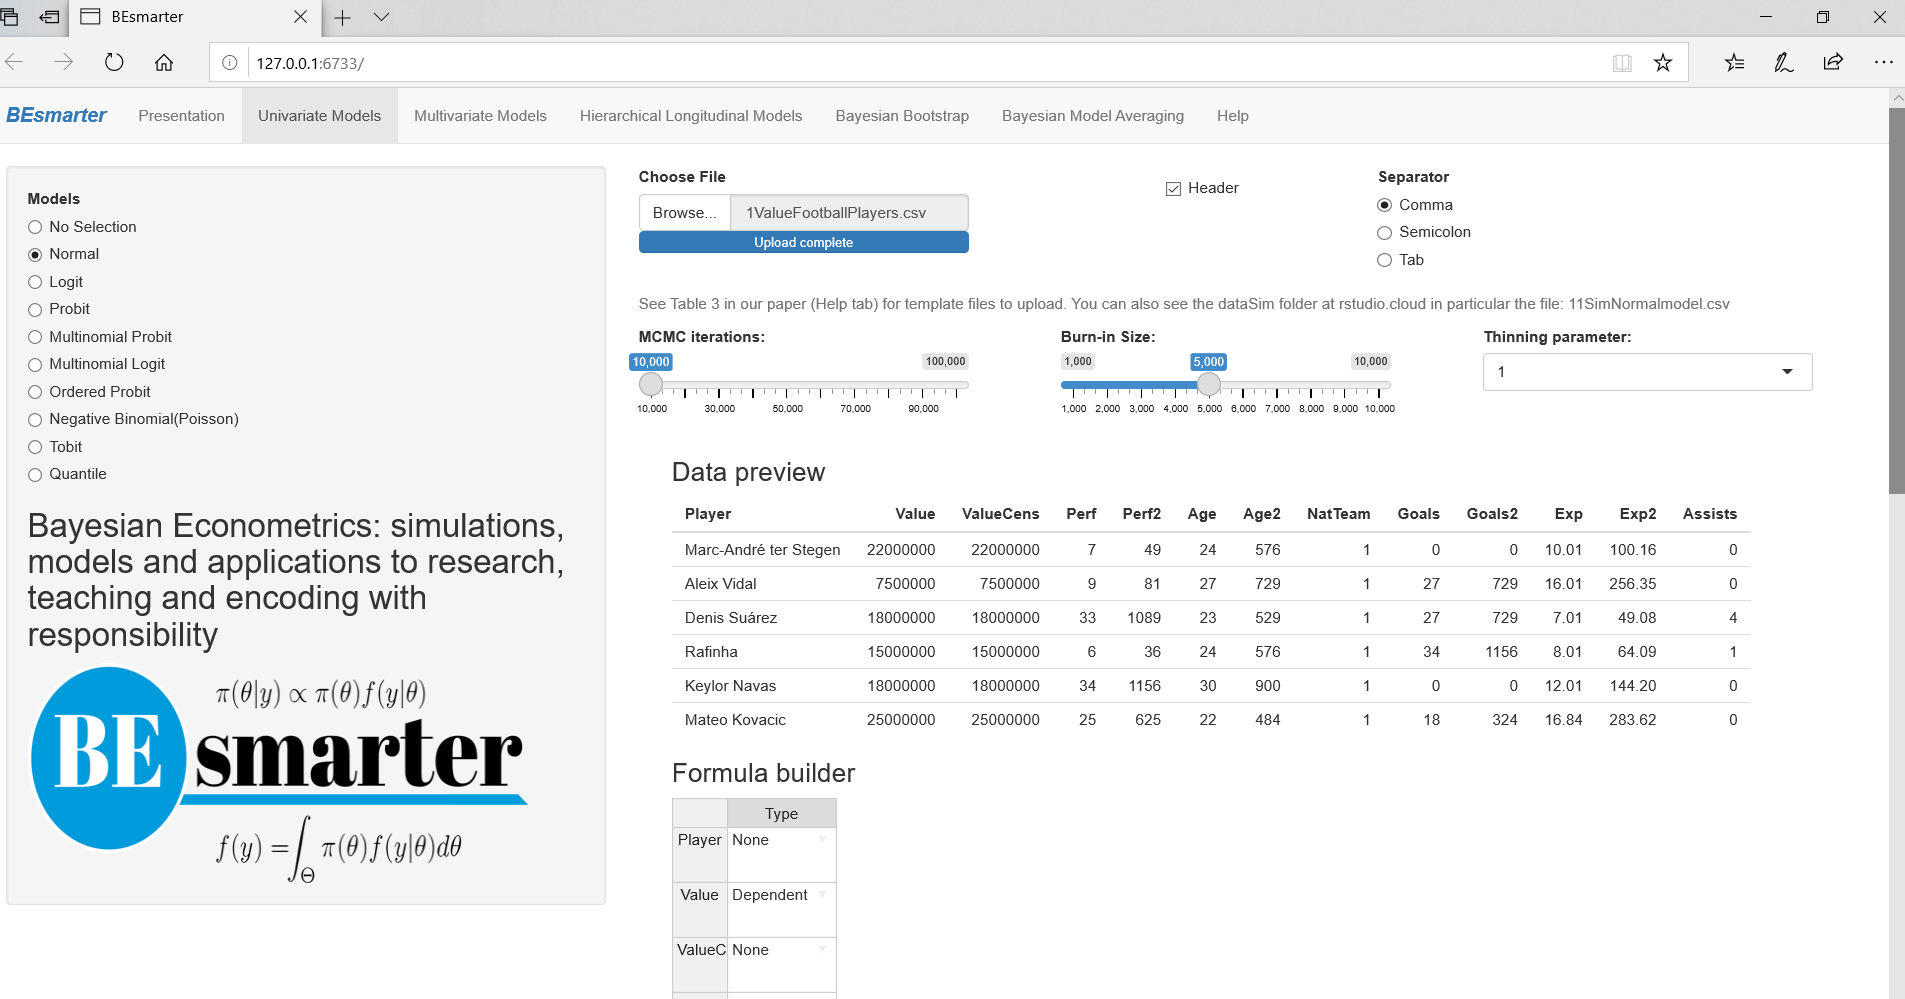
\includegraphics[width=340pt, height=130pt]{Chapters/chapterGUI/figures/Figure1.png}
	\caption[List of figure caption goes here]{Display of our graphical user interface.}\label{fig61}
\end{figure}

\section{Univariate models}\label{secGUI2}
After our GUI is deployed (see Figure \ref{fig61}), the user should select \textit{Univariate Models} in the top panel. Then, the Figure \ref{fig62} is displayed, and the user can see the radio button on the left hand side that shows the specific models inside this generic class. In particular, users can see that the normal model is selected from inside the class of univariate models.

\begin{figure}
	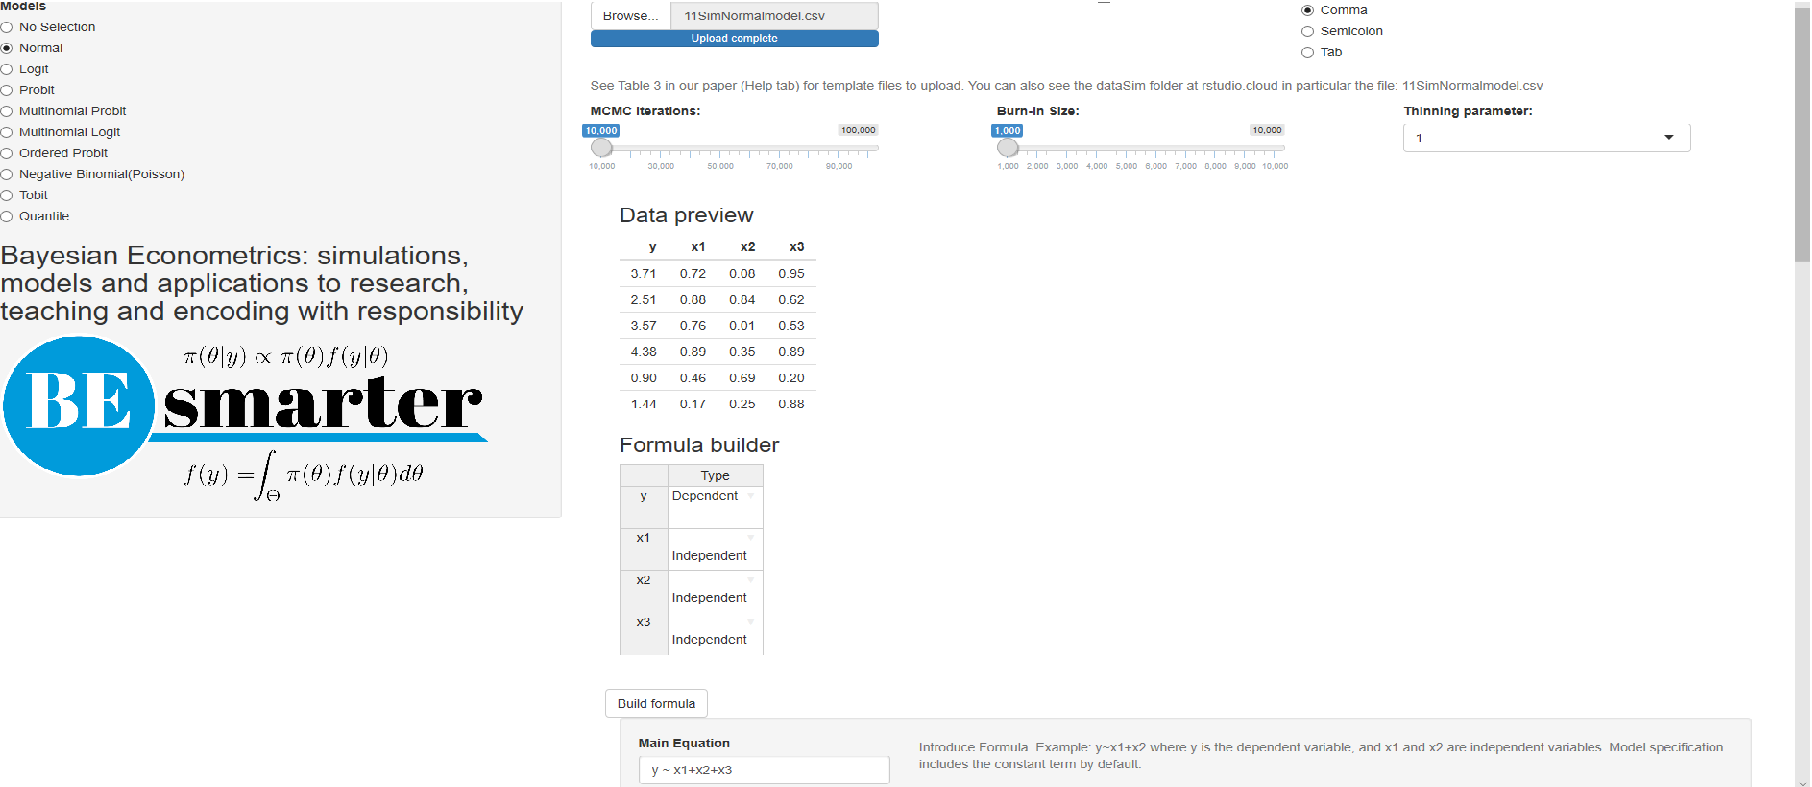
\includegraphics[width=340pt, height=130pt]{Chapters/chapterGUI/figures/Figure2.png}
	%%\centerline{\epsfig{/Chapters/chapter1/figures/cat.eps,width=.8\textheight,height=.4\textwidth}}
	\caption[List of figure caption goes here]{Univariate models: Specification.}\label{fig62}
\end{figure}

Then, the right hand side panel displays a widget to upload the input dataset, which should be a \textit{csv} file with headers in the first row. Users also should select the kind of separator used in the input file: comma, semicolon, or tab (use the folders \textbf{DataSim} and \textbf{DataApp} for the input file templates). Once users upload the dataset, they can see a data preview. Range sliders help to set the number of iterations of the Markov chain Monte Carlo algorithm, the amount of burn-in, and the thinning parameter can be selected as well (see next chapters of this second part of the book for technical details). After this, users should specify the equation. This can be done with the formula builder, where users can select the dependent variable, and the independent variables, and then click on the \textit{Build formula} tab. Users can see in the \textit{Main Equation} space the formula expressed in the format used by \textbf{R} software (see Main equation box in Figure \ref{fig62}, $y\sim x1+x2+x3$). Users can modify this if necessary, for instance, including higher order or interaction terms, other transformations are also allowed. This is done directly in the \textit{Main Equation} space taking into account that this extra terms should follow formula command structure.\footnote{See \textbf{https://www.rdocumentation.org/packages/stats/versions/3.6.2/topics/formula}} Note that the class of univariate models includes the intercept by default, except ordered probit, where the specification has to do this explicitly, that is, ordered probit models do not admit an intercept, for \textit{identification} issues (see details below).\footnote{An \textit{identification} issue means that multiple values for the model parameters give rise to the same value for the likelihood function.} Hence, users should write down specifically this fact ($y\sim x1+x2+x3-1$). Finally, users should define the hyperparameters of the prior; for instance, in the normal-inverse gamma model, these are the mean vector, covariance matrix, shape, and scale parameters (see Figure \ref{fig63}). However, users should take into account that our GUI has \textit{non-informative} hyperparameters by default in all our modelling frameworks, so the last part is not a requirement.

\begin{figure}
	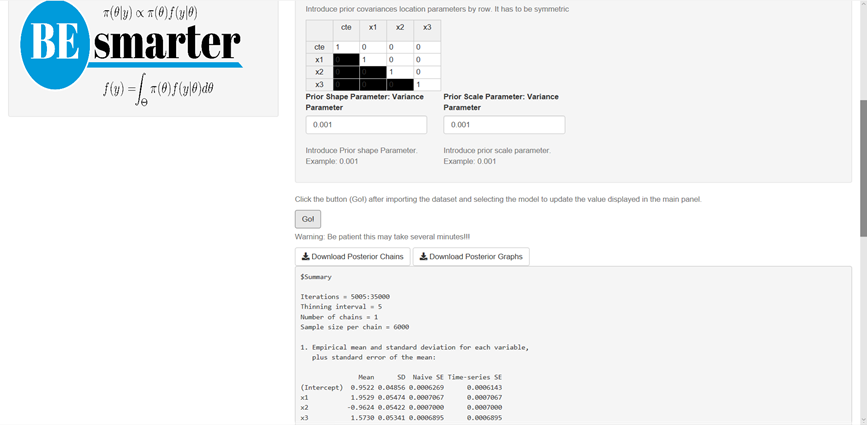
\includegraphics[width=340pt, height=130pt]{Chapters/chapterGUI/figures/Figure3.png}
	%%\centerline{\epsfig{/Chapters/chapter1/figures/cat.eps,width=.8\textheight,height=.4\textwidth}}
	\caption[List of figure caption goes here]{Univariate models: Results.}\label{fig63}
\end{figure}

After this specification process, users should click the \textit{Go!} button to initiate the estimation. Our GUI displays the summary statistics and convergence diagnostics after this process is finished (see Figure \ref{fig63}). There are also widgets to download posterior chains (\textit{csv} file) and graphs (\textit{pdf} and \textit{eps} files). Note that the order of the coefficients in the results (summary, posterior chains, and graphs) is first for the location parameters, and then for the scale parameters.

Multinomial models (probit and logit) require a dataset file to have in the first column the dependent variable, then alternative specific regressors (for instance alternatives' prices), and finally, non-alternative regressors (for instance, income). The formula builder specifies the dependent variable, and independent variables that are alternative specific and non-alternative specific (see technical details in next chapter). Specification also requires defining the base category, number of alternatives (this is also required in ordered probit), number of alternative specific regressors, and number of non-alternative regressors (see Figure \ref{fig64}). Multinomial logit also allows defining a tuning parameter, the number of degrees of freedom in this case, for the Metropolis--Hastings algorithm (see technical details in next chapter). This is a feature in our GUI when the estimation of the models is based on the Metropolis--Hastings algorithm. The order of the coefficients in the results of these models is first the intercepts (cte$_l$ appearing in the summary display, $l$-th alternative), and then the non-alternative specific regressors (NAS$_{jl}$ appearing in the summary display, $l$-th alternative and $j$-th non-alternative regressor), and lastly, the coefficients for the alternative specific regressors (AS$_{j}$ appearing in the summary display, $j$-th alternative specific regressor). Note that the non-alternative specific regressors associated with the base category are equal to zero (they do not appear in the results). In addition, some coefficients of the main diagonal of the covariance matrix are constant due to identification issues in multinomial and multivariate probit models.

\begin{figure}
	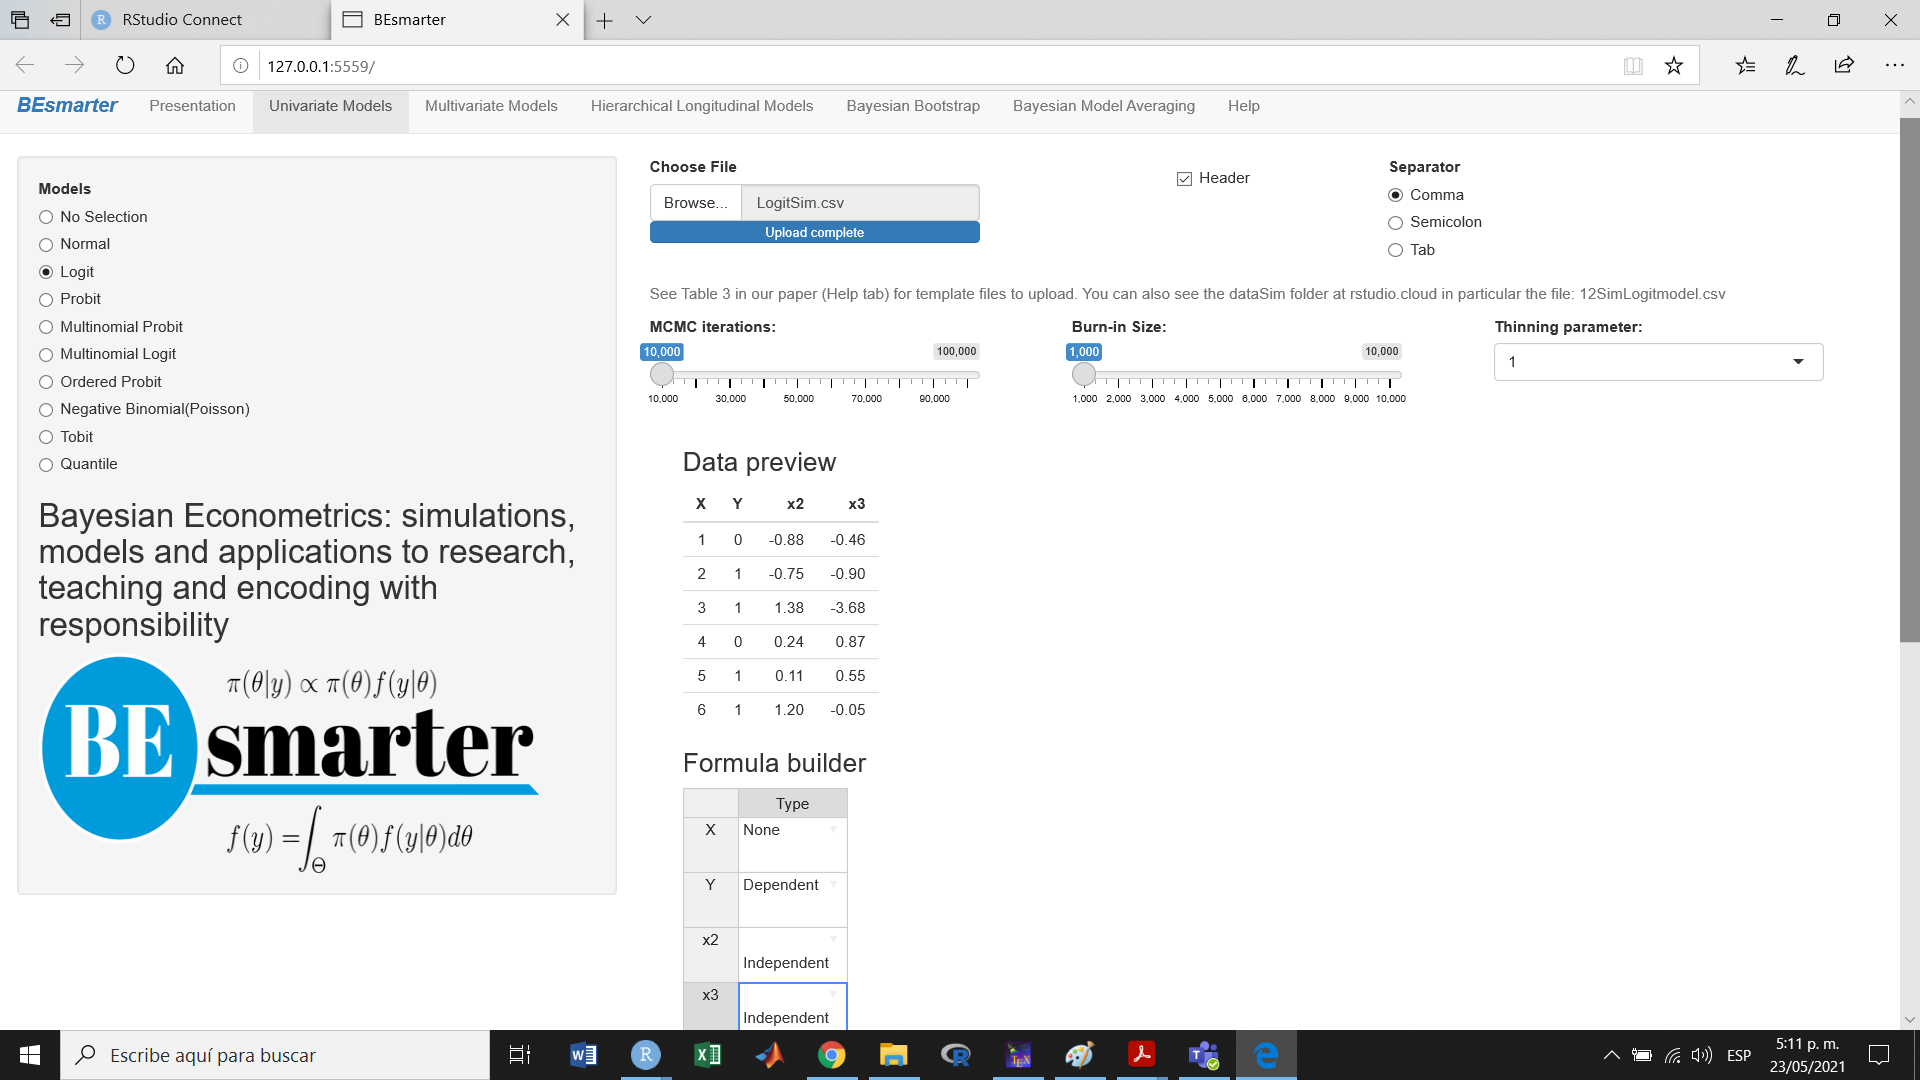
\includegraphics[width=340pt, height=130pt]{Chapters/chapterGUI/figures/Figure4.png}
	%%\centerline{\epsfig{/Chapters/chapter1/figures/cat.eps,width=.8\textheight,height=.4\textwidth}}
	\caption[List of figure caption goes here]{Univariate models: Multinomial.}\label{fig64}
\end{figure}

In the case of the negative binomial model, users should set a dispersion parameter (see the negative binomial model in the next chapter). User should also set the censorship points and quantiles in the Tobit and quantile models, respectively.

Bayesian bootstrap only requires uploading a dataset, specifying the number of iterations of the MCMC, the resampling size, and the equation (see Figure \ref{fig65}).
The input file has the same structure as the file used in the univariate normal model.

\begin{figure}
	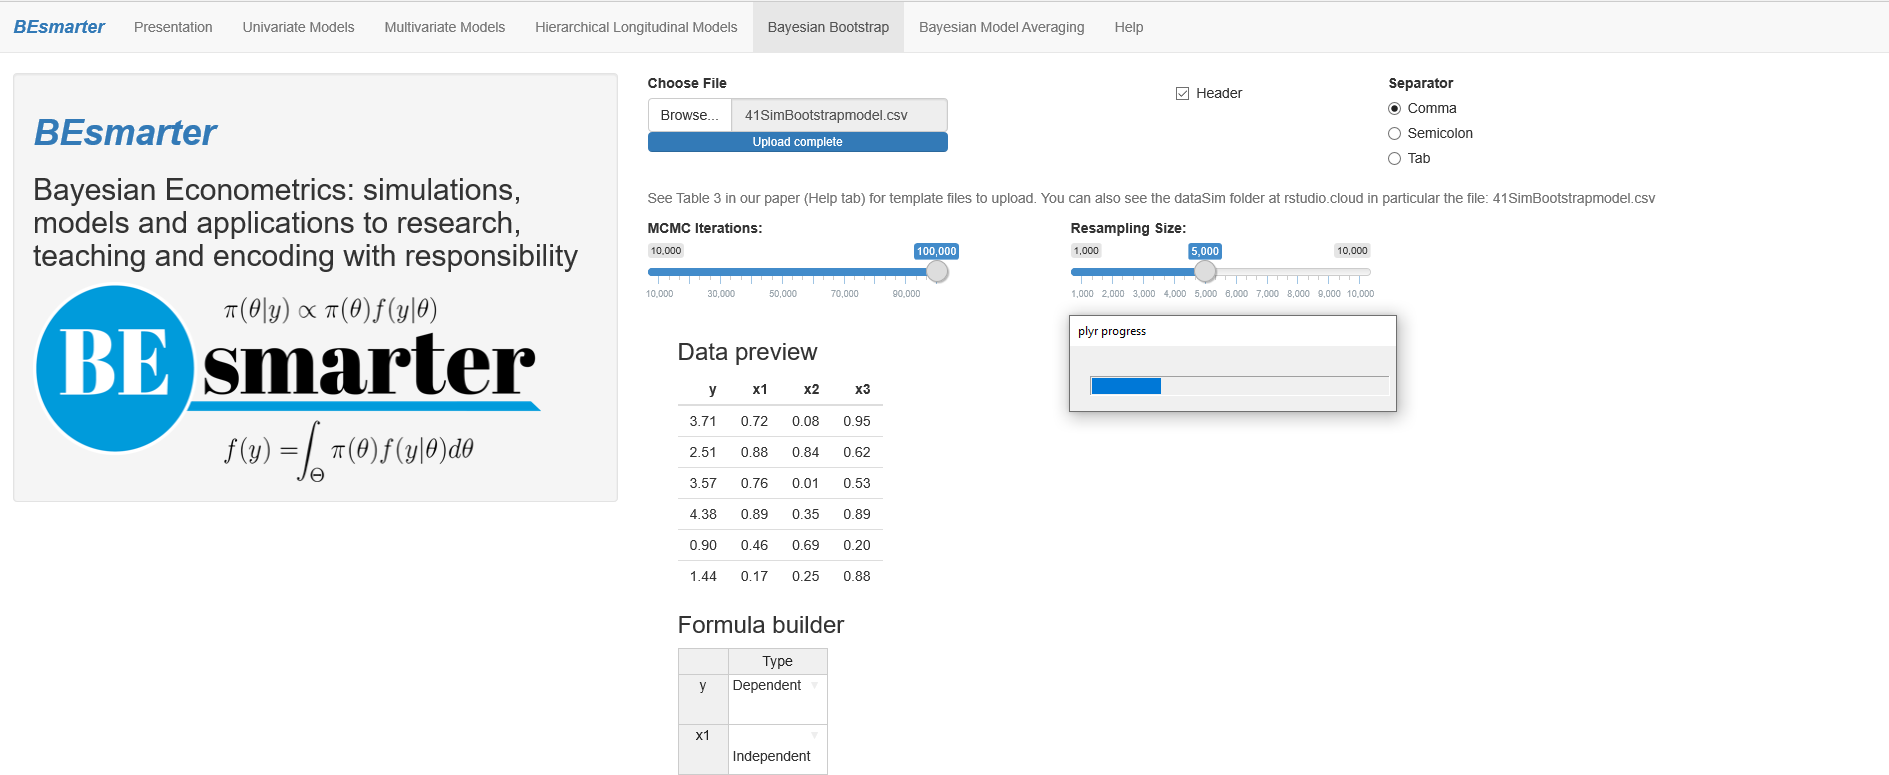
\includegraphics[width=340pt, height=130pt]{Chapters/chapterGUI/figures/Figure5.png}
	%%\centerline{\epsfig{/Chapters/chapter1/figures/cat.eps,width=.8\textheight,height=.4\textwidth}}
	\caption[List of figure caption goes here]{Univariate models: Bootstrap.}\label{fig65}
\end{figure}  

\section{Multivariate models}\label{secGUI3}
After our GUI is deployed (see Figure \ref{fig61}), the user should select \textit{Multivariate Models} in the top panel. Then, the Figure \ref{fig66} is displayed, and the user can see the radio button on the left hand side that shows the specific models inside this generic class.

Figure \ref{fig66} displays the multivariate regression setting. In this case, the input file should have first the dependent variables, and then the regressors. If there are intercepts in each equation, there should be a column of 1's after the dependent variables in the input file. The user also has to set the number of dependent variables, the number of regressors, if necessary include the intercept, and the values of the hyperparameters (see Figure \ref{fig66}).

\begin{figure}
	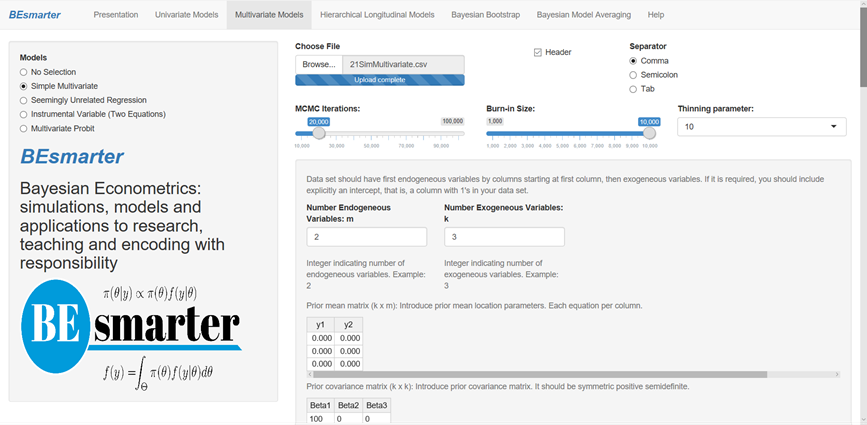
\includegraphics[width=340pt, height=130pt]{Chapters/chapterGUI/figures/Figure6.png}
	%%\centerline{\epsfig{/Chapters/chapter1/figures/cat.eps,width=.8\textheight,height=.4\textwidth}}
	\caption[List of figure caption goes here]{Multivariate models: Simple multivariate.}\label{fig66}
\end{figure}

The input file in seemingly unrelated regressions should have first the dependent variables, and then the regressors by equation, including the intercept in each equation if necessary (column of 1's). Users should define the number of dependent variables (equations), the number of total regressors, that is, the sum of all regressors associated with the equation (if necessary include intercepts, each intercept is an additional regressor), and the number of regressors by equation (if necessary include the intercept). Users can also set the values  of the hyperparameters if there is prior information.

The results of the simple multivariate and seemingly unrelated regressions show first the posterior location parameters by equation, and then the posterior covariance matrix.

In the instrumental variable setting, users should specify the main equation and the instrumental equation. This setting includes intercepts by default. The first variable on the right hand side in the main equation has to be the variable with endogeneity issues. In the instrumental equation box, the dependent variable is the variable with endogeneity issues as a function of the instruments. Users can also specify the values of the hyperparameters if they have prior information. The input file should have the dependent variable, the endogenous regressor, the instruments, and the exogenous regressors. The results first list the posterior estimates of the endogenous regressor, then the location parameters of the auxiliary regression (instrumental equation), and the location parameters of the exogenous regressors. Last is the posterior covariance matrix.

\begin{figure}
	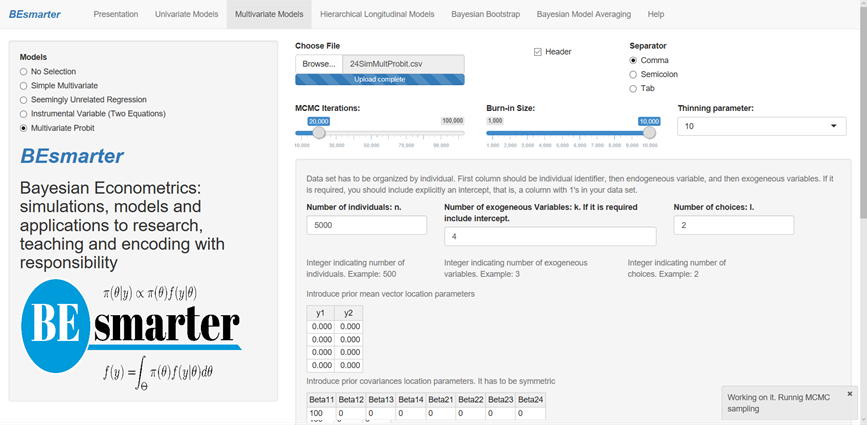
\includegraphics[width=340pt, height=130pt]{Chapters/chapterGUI/figures/Figure7.png}
	%%\centerline{\epsfig{/Chapters/chapter1/figures/cat.eps,width=.8\textheight,height=.4\textwidth}}
	\caption[List of figure caption goes here]{Multivariate models: Multivariate probit.}\label{fig67}
\end{figure} 

The multivariate probit model requires an input dataset ordered by unit, for instance three choices implies repeat each unit three times. The first column has to be the identification of each unit; users should use ordered integers, then the dependent variable, just one vector, composed of 0's and 1's, then the regressors, which should include a column of 1's for the intercepts. Users should set the number of units, number of regressors, and number of choices (see Figure \ref{fig67}). The results first display the posterior location parameters by equation, and then the posterior covariance matrix.

\section{Time series model}\label{secGUI4}

\section{Longitudinal/panel models}\label{secGUI5}
After our GUI is deployed (see Figure \ref{fig61}), the user should select \textit{Hierarchical Longitudinal Models} in the top panel. Then, the Figure \ref{fig68} is displayed, and the user can see the radio button on the left hand side that shows the specific models inside this generic class.


The hierarchical longitudinal models tab allows for estimating models that account for within-subject correlation when the dependent variable is continuous (Normal), binary (Logit), or a count (Poisson).

The input files for hierarchical longitudinal models should have first the dependent variable, then the regressors and a cross sectional identifier ($i=1,2,\dots,N$). It is not a requirement to have a balanced dataset: $T_i$ can be different for each $i$ (see Chapter \ref{chap9} for technical details). Users can see templates of datasets in the folders \textbf{DataSim} (see Table \ref{tab:simdata} for details), and \textbf{DataApp} (see Table \ref{tab:appdata} for details) of our \textit{GitHub} repository. Users should also specify the fixed part equation and the random part equation,
both in \textbf{R} format. In case of only requiring random intercepts, do not introduce anything in the latter part (see Figure \ref{fig68}). Users should also type the name of the cross sectional identifier variable. The results displayed and the posterior graphs are associated with the fixed effects and covariance matrix. However, users can download the posterior chains of all posterior estimates: fixed and random effects, and covariance matrix.

\begin{figure}
	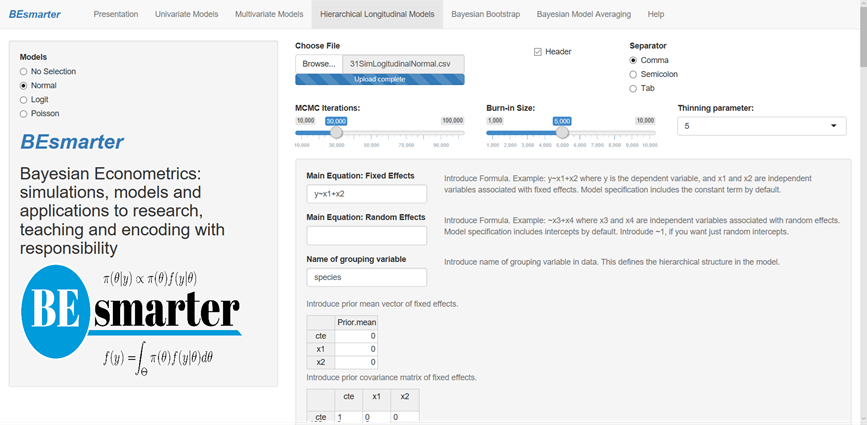
\includegraphics[width=340pt, height=130pt]{Chapters/chapterGUI/figures/Figure8.png}
	%%\centerline{\epsfig{/Chapters/chapter1/figures/cat.eps,width=.8\textheight,height=.4\textwidth}}
	\caption[List of figure caption goes here]{Hierarchical longitudinal models: Specification.}\label{fig68}
\end{figure} 

\section{Bayesian model average}\label{secGUI6}

After our GUI is deployed (see Figure \ref{fig61}), the user should select \textit{Bayesian Model Averaging} in the top panel. Then, the Figure \ref{fig69} is displayed, and the user can see the radio button on the left hand side that shows the specific models inside this generic class.

Bayesian model averaging based on a Gaussian distribution can be carried out using the Bayesian information criterion (BIC) approximation, Markov chain Monte Carlo model composition (MC3), or instrumental variables (see Figure \ref{fig69}). The former two approaches require an input dataset where the first column is the dependent variable, and then, the potentially important regressors.
Users should set the band width model selection parameter ($O_R$) and number of iterations for BIC and MC3, respectively (see Chapter \ref{chap10} for technical details). The results include the posterior inclusion probability ($p!=0$), expected value (EV), and standard deviation (SD) of the coefficients associated with each regressor. The BIC framework also displays the most relevant models, including the number of regressors, the coefficient of determination ($R^2$), the BIC, and the posterior model probability. Users can download two \textit{csv} files: \textit{Best models} and \textit{Descriptive statistics coefficients}. The former is a 0-1 matrix such that the columns are the regressors and the rows are the models; a 1 indicates the presence of a specific regressor in a specific model, 0 otherwise. Note that the last column of this file is the posterior model probability for each model (row). The latter file shows the posterior inclusion probabilities, expected values, and standard deviations associated with each regressor, taking into account the BMA procedure based on the best models.

\begin{figure}
	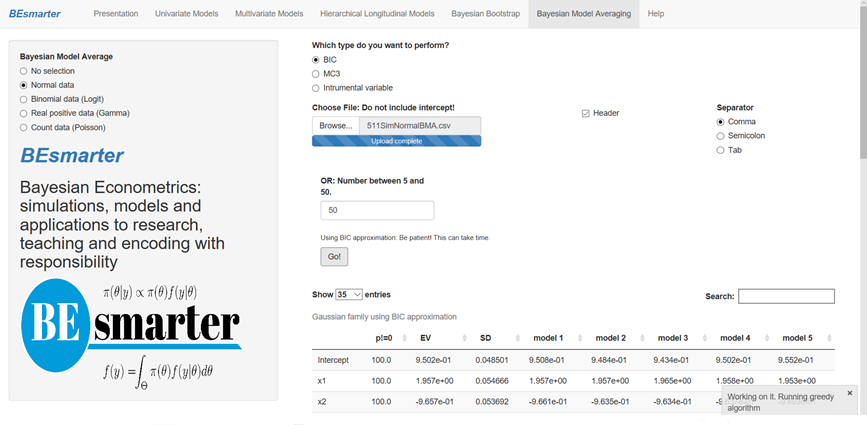
\includegraphics[width=340pt, height=130pt]{Chapters/chapterGUI/figures/Figure9.png}
	%%\centerline{\epsfig{/Chapters/chapter1/figures/cat.eps,width=.8\textheight,height=.4\textwidth}}
	\caption[List of figure caption goes here]{Bayesian model averaging: Specification and results.}\label{fig69}
\end{figure} 

Bayesian model averaging with endogeneity issues requires two input files. The first one has the dependent variable in the first column, the next columns are the regressors with endogeneity issues, and then the exogeneous regressors. The user should include a column of 1's if an intercept is required. The second input file has all the instruments. Users should also introduce the number of regressors with endogeneity issues (see Figure \ref{fig610}).

\begin{figure}
	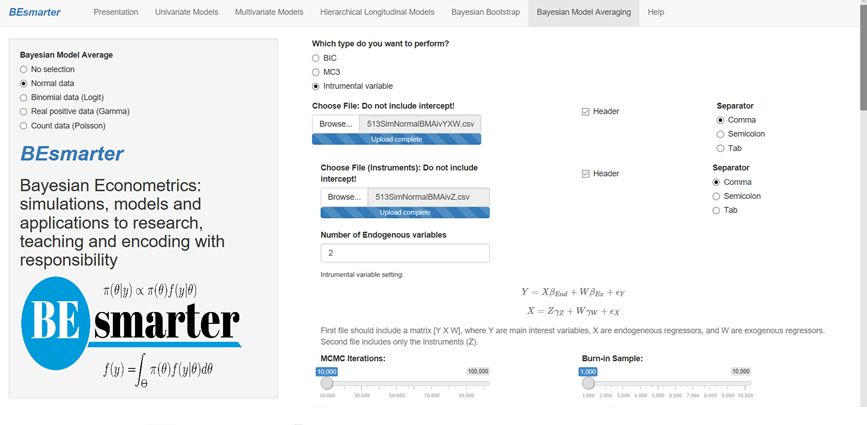
\includegraphics[width=340pt, height=130pt]{Chapters/chapterGUI/figures/Figure10.png}
	%%\centerline{\epsfig{/Chapters/chapter1/figures/cat.eps,width=.8\textheight,height=.4\textwidth}}
	\caption[List of figure caption goes here]{Bayesian model averaging: Instrumental variable specification.}\label{fig610}
\end{figure} 

The results include the posterior inclusion probabilities and expected values for each regressor. The user can find the results of the main equation, and then of the auxiliary equations. Users can download \textit{csv} files of BMA results for both the second stage (main equation)  and the first stage (auxiliary equations). In addition, users can download the posterior chains of the location parameters of the main equation, $\beta_{l}$, $l=1,2,\dots,dim\left\{\bm{\beta}\right\}$, the location parameters of the auxiliary equations, $\gamma_{j,i}$, $j=1,2,\dots,dim\left\{\bm{\beta}_s\right\}$ where $dim\left\{\bm{\beta}_s\right\}$ is the number of regressors with endogeneity issues, $i=1,2,\dots,dim\left\{\bm{\gamma}\right\}$, where $dim\left\{\bm{\gamma}\right\}$ is the number of regressors in the auxiliary regressors (exogeneous regressors + instruments), and the elements of the covariance matrix $\sigma_{j,k}$ (see Chapter \ref{chap10} for technical details).

Bayesian model averaging based on BIC approximation for non-linear models, Logit, Gamma, and Poisson, requires an input dataset where the first column is the dependent variable, and the other columns are the potentially relevant regressors. Users should specify the band width model selection parameters, which are also referred to as Occam's window parameters ($O_R$ and $O_L$). Our GUI displays the posterior inclusion probabilities ($p!=0$), the expected value of the posterior coefficients (EV), and the standard deviation (SD). In addition, users can see the results associated with the models with the highest posterior model probabilities, and download \textit{csv} files with the results of specifications of the best models, and descriptive statistics of the posterior coefficients from the BMA procedure. These files are similar to the results of the BIC approximation of the Gaussian model.

\section{Warning}\label{secGUI7}

Users should also note that sometimes our GUI shuts down. In our experience, this is due to computational issues using the implicit commands that we call when estimating some models, for instance, computationally singular systems, missing values where TRUE/FALSE needed, L-BFGS-B needs finite values of ``fn'', NA/NaN/Inf values, or Error in backsolve. Sometimes these issues can be solved by adjusting the dataset, for instance, avoiding high levels of multicollinearity. It should also be taken into account that when warning messages are displayed in our GUI, there is a high chance that there are convergence issues of the posterior chains. So, the results are not trustworthy. Users can identify these problems by checking the console of their \textit{RStudio} sections, where the specific folder/file where the issue happened is specified. In any case, we would appreciate your feedback to improve and enhance our GUI.

We also should say there are many ways to improve the codes that we present in the following five chapters. For instance, the \textit{MCMCpack} and \textit{bayesm} packages perform most of the matrix operations in C++ using the \textit{rcpp} package. This substantially speeds up the algorithms compared with the codes that we present in the next chapters. We could improve the computational times of our codes using parallel computing and the \textit{rcpp} package, but this requires more advanced skills that we do not cover in this book.
